% !TeX document-id = {d8a08665-68b2-4c28-8b7c-81fa3895c963}
% !TEX TS-program = pdflatexmk
\documentclass[10pt,a4paper]{article}
\usepackage[english]{babel}
\usepackage[latin1]{inputenc}
\usepackage{lipsum}
\usepackage{authblk}
\usepackage{amsmath}
\usepackage{amsfonts}
\usepackage{amssymb}
\usepackage{polski}
\usepackage{graphicx}
\usepackage{cite}
\usepackage{listings}
\usepackage{float}
\selectlanguage{english}
\begin{document}
	
	\begin{figure}[H]
		\centering
		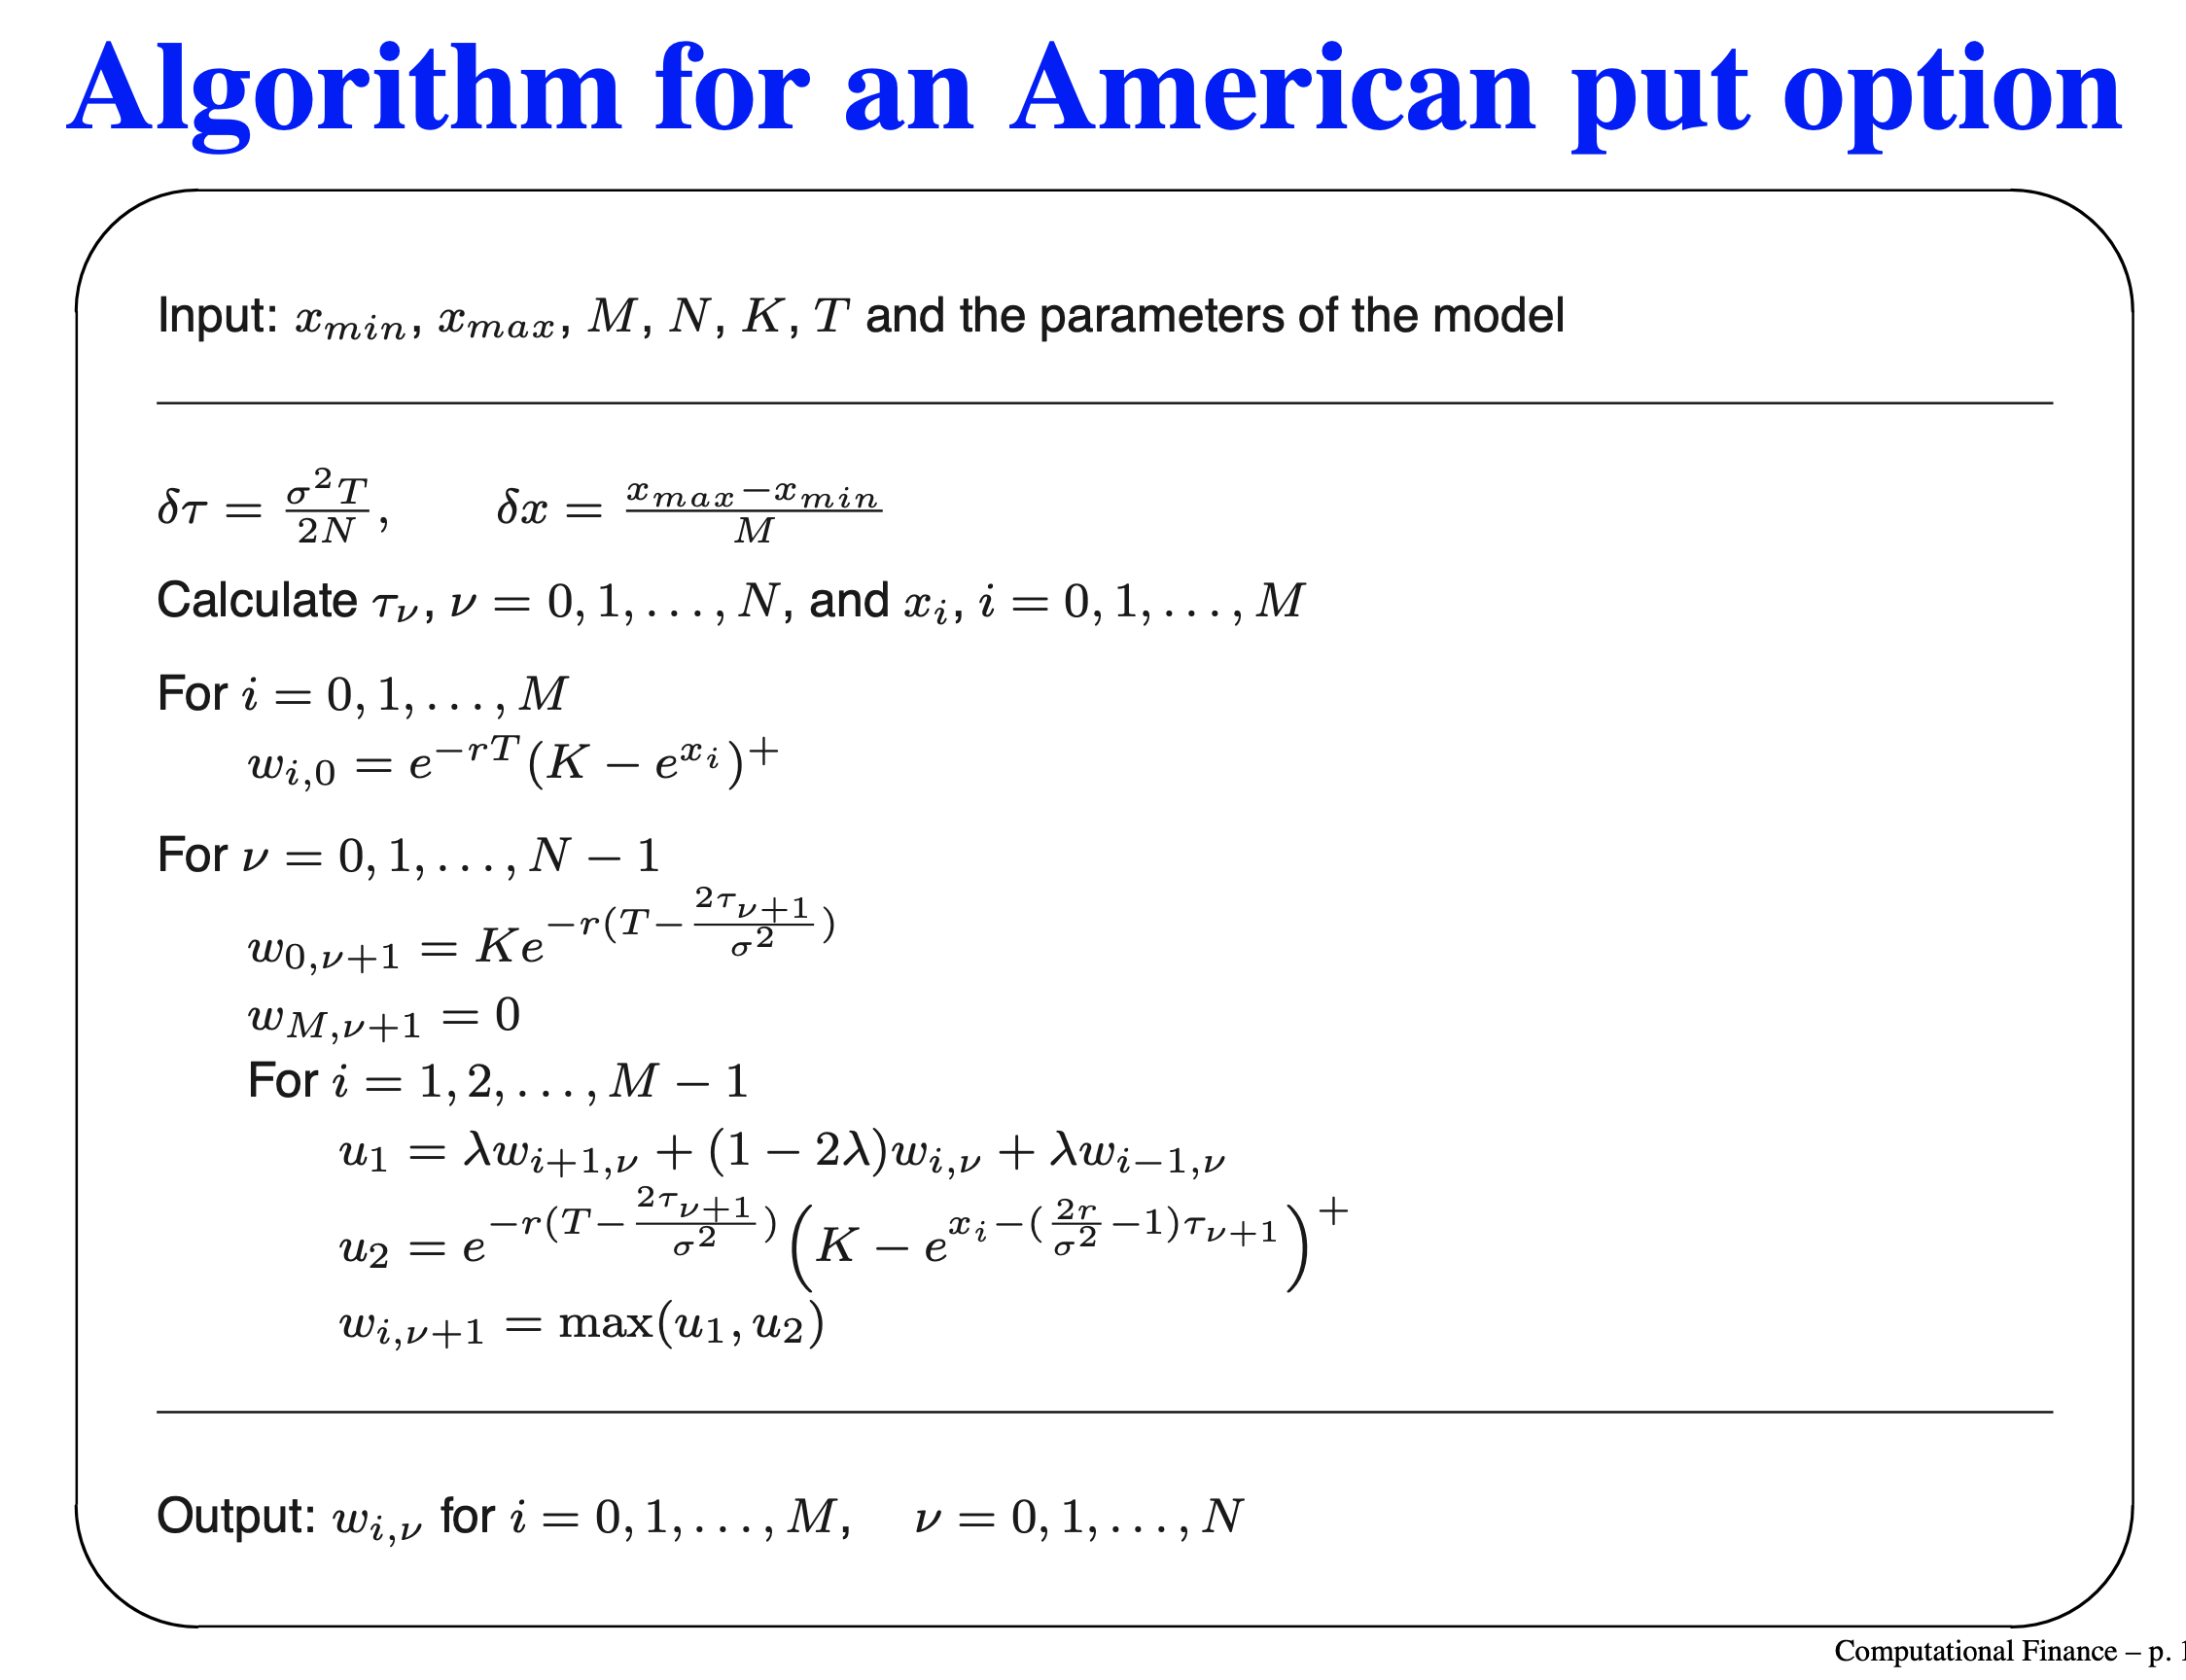
\includegraphics[width = 1.0\linewidth]{palczewski.png}
		\caption[Algorithm - American BS]{Algorithm - American BS}
		\label{fig:Al}
	\end{figure}
	
	\begin{figure}[H]
		\centering
		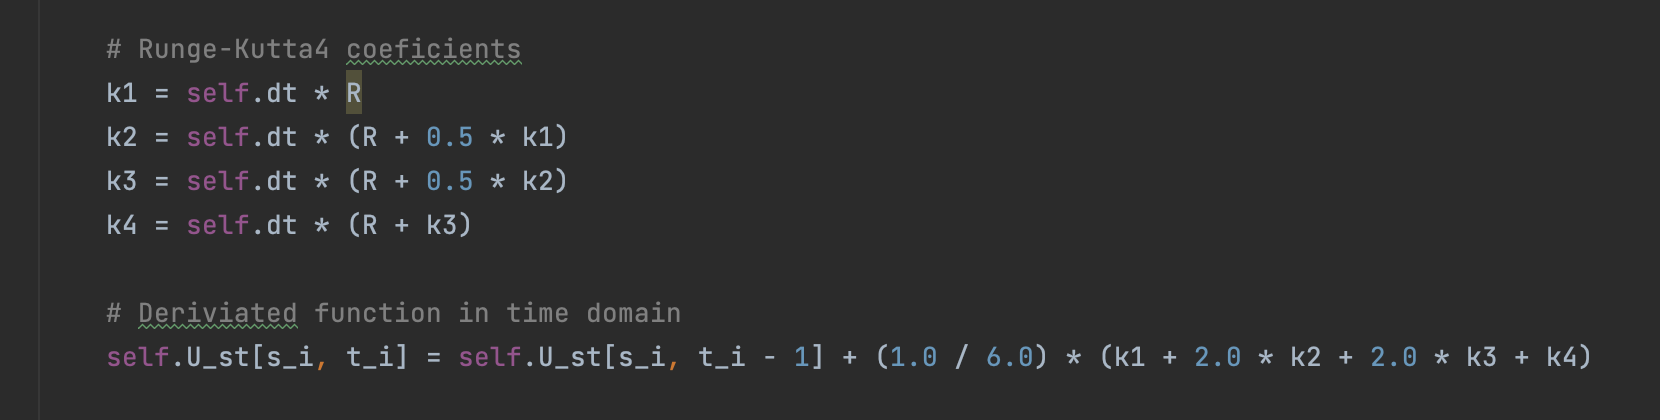
\includegraphics[width = 1.0\linewidth]{european.png}
		\caption[European Option computation]{European Option computation}
		\label{fig:Eu}
	\end{figure}

	\begin{figure}[H]
		\centering
		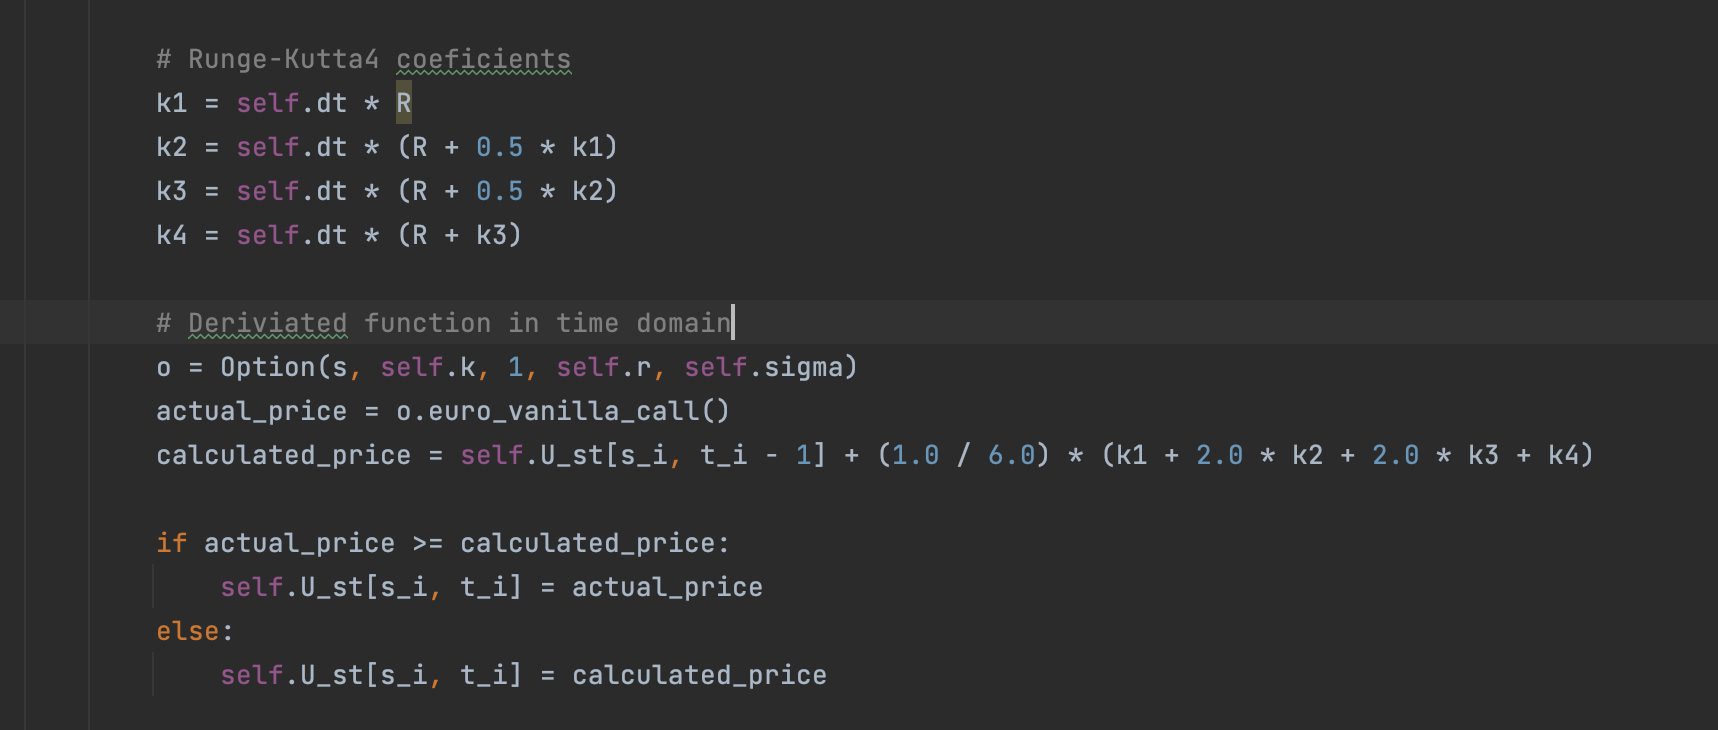
\includegraphics[width = 1.0\linewidth]{american.png}
		\caption[American Option computation]{American Option computation}
		\label{fig:Am}
	\end{figure}
	
	\begin{figure}[H]
		\centering
		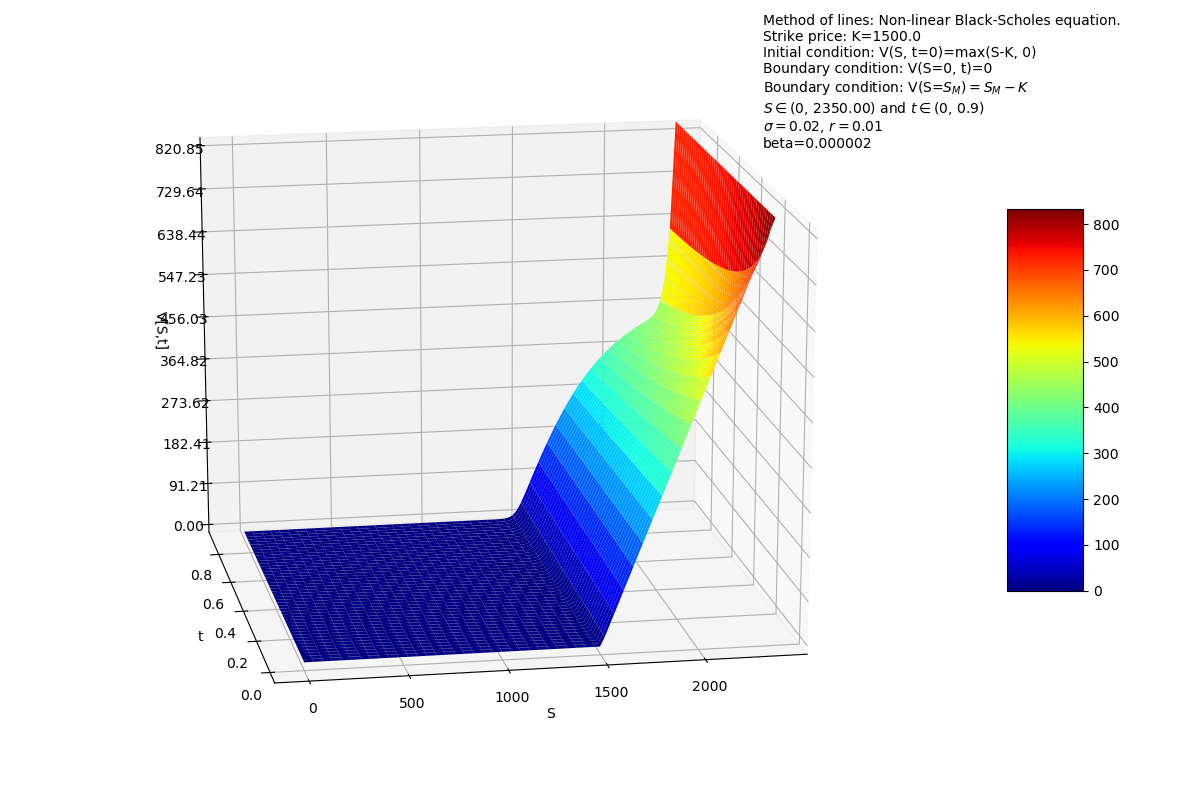
\includegraphics[width = 1.0\linewidth]{Black-Scholes_K1500.0_sigma0.02_r0.01_beta2e-06_T0.9_nonlinear_european.png}
		\caption[European Option - non-linear BS]{European Option - non-linear BS}
		\label{fig:E}
	\end{figure}

	\begin{figure}[H]
	\centering
	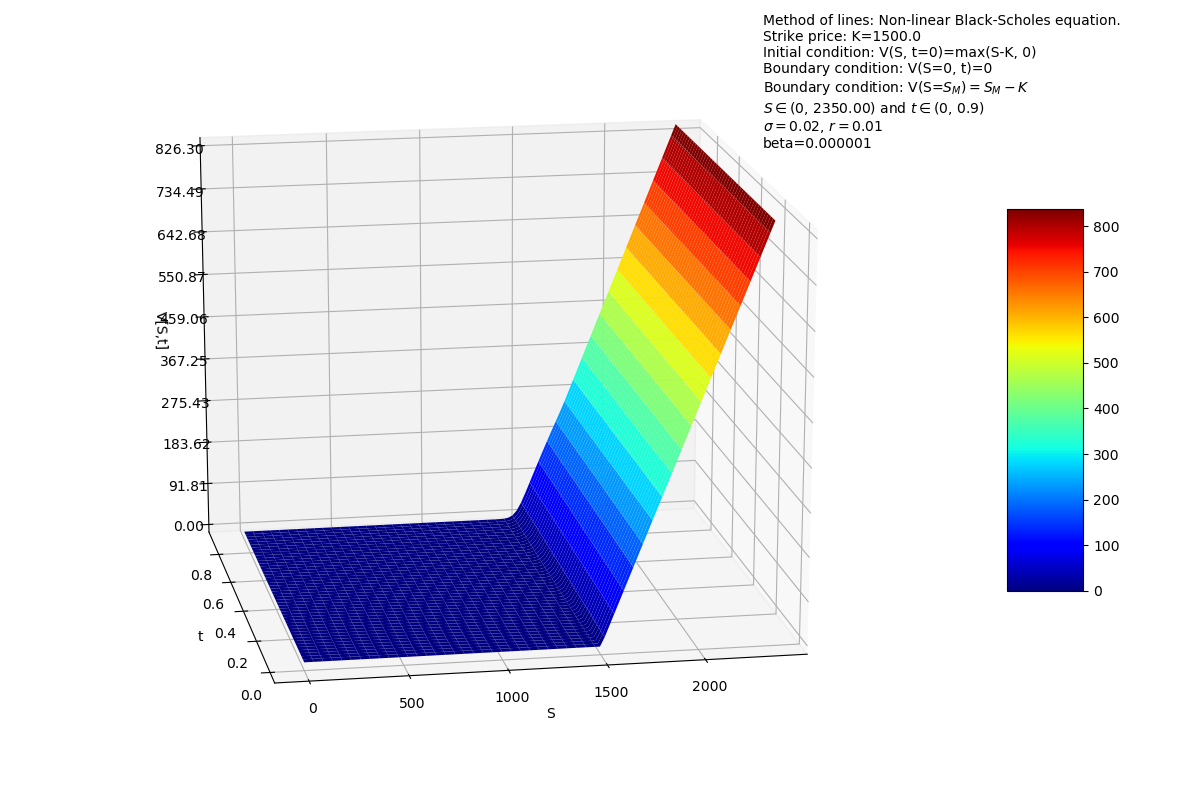
\includegraphics[width = 1.0\linewidth]{Black-Scholes_K1500.0_sigma0.02_r0.01_beta1e-06_T0.9_nonlinear_american.png}
	\caption[American Option - non-linear BS]{American Option - non-linear BS}
	\label{fig:A}
   \end{figure}

  	\begin{figure}[H]
  	\centering
  	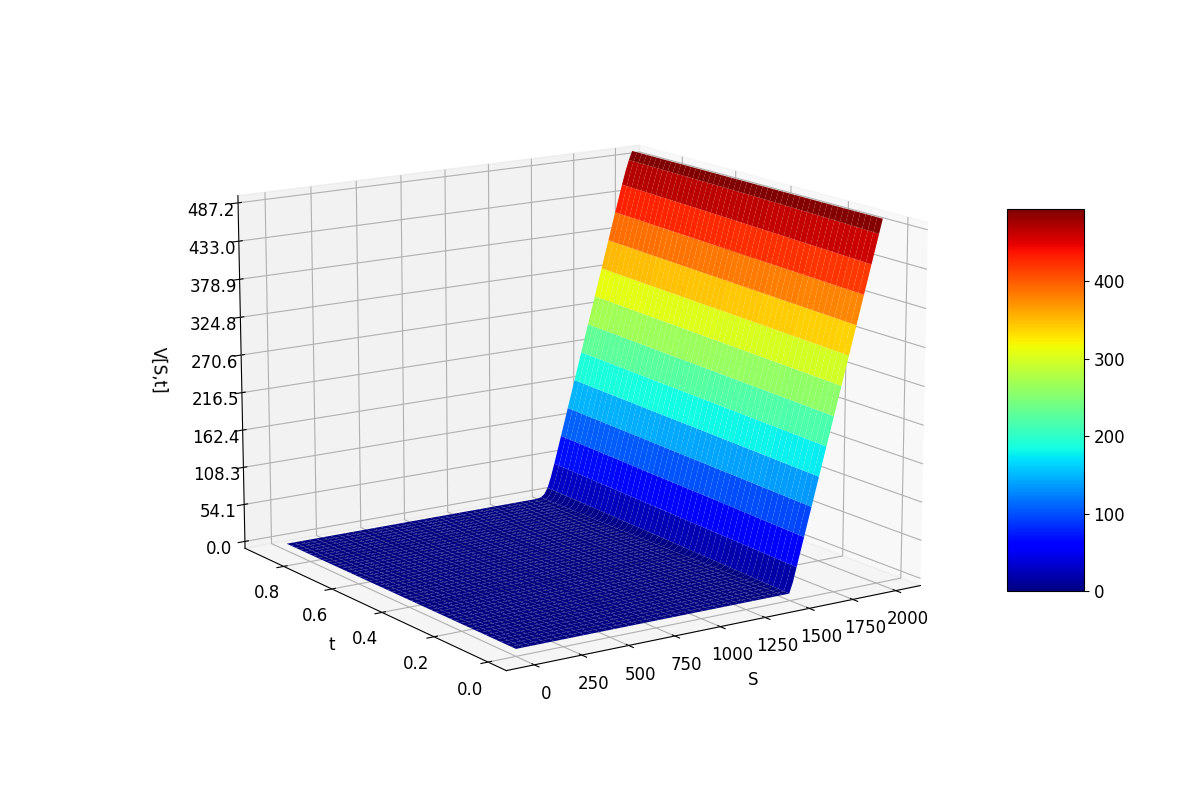
\includegraphics[width = 1.0\linewidth]{Black-Scholes_K1500.0_sigma0.02_r0.01_T0.9_linear_european.png}
  	\caption[European Option - linear BS]{European Option - linear BS}
  	\label{fig:E}
  \end{figure}
  
  \begin{figure}[H]
  	\centering
  	\includegraphics[width = 1.0\linewidth]{Black-Scholes_K1500.0_sigma0.02_r0.01_T0.9_linear_american.png}
  	\caption[American Option - linear BS]{American Option - linear BS}
  	\label{fig:A}
  \end{figure}
\end{document}